% Chapter 1

\chapter{State of the art}

\label{State of the art}

\cite{survey1}
\section{Botnets}
\cite{survey2}
As stated in the introduction botnets are an important problem for anyone involved somehow with the internet. They can result in great economic damage.
\cite{report1} 
Especially with their continuous improvement to become more resilient and powerful which makes them an even more important threat.\\\\
\cite{pheonix} 
Botnets can become very lucrative and can infect very large amount of devices resulting in scary tool. Here are some examples of the magnitude they can reach: \textbf{Flashback} with 600k compromised targets, \textbf{Grum} with 840k compromised devices and sending 40 Billion spam emails per month, \textbf{TDL-4} with 4.5 Million victims in first the 3 months and \textbf{Gameover ZeuS} with 1 Million infections, because of its resilience mechanisms this botnet was one of the hardest to take down.\\\\
\cite{survey2}
The reason botnets are still an ongoing research topic is that there isn't a complete solution for their detection and mitigation. Researchers and organisations have to keep working to keep updated with all the new flavors criminals bring to the market.
\subsection{Definition}
% WHAT IS A BOTNET?
\cite{memoire1}
\cite{detection1}
\paragraph{What is a botnet?} A botnet is a network of infected machines with programs called bots, these bots owned and controlled by a remote attacker called the botmaster. Users get infected via the same vector attacks used by malware, email attachment, malicious website, unaware download, etc. When bots usually infect these machines in stealthy manner, staying as unnoticeable as possible. The control of such bots is done through the Command and Control (CnC) server. The CnC server allows the master to issue commands to and receives responses from individual bots or aggregations of bots. These exchanges are done to update the software of the malware, execute attacks, exfiltrate data and more actions explained down below.
\cite{survey3}

%WHAT IS A BOT?
\cite{honeynet}
\paragraph{What is a bot?} Bots are small programs allowing to remotely control and perform commands on computers. They are the foundation of botnets. The paper presented by the SANS institute considers two types of bots. Bots used to perpetuate attacks, bots used for their content and both. \cite{tracking}
\cite{bot-com}
A clear distinction between a bot agent and a common piece of malware lies within a bot's ability to communicate with a Command-and-Control (CnC) infrastructure. CnC allows a bot agent to receive new instructions and malicious capabilities, as dictated by a remote criminal entity. This compromised host then can be used as an unwilling participant in Internet crime as soon as it is linked into a botnet via that same CnC.\\
These programs are embedded with port scanning, vulnerability scanning, exploitation kits and payloads that allow them to spread the botnet and infect their victims.\\
There are many different families of bots, some very modular such as the Agobot others less complete but easier to use such as the SDBot family. Bots families are also classified depending on the channel type and attack type, for example GT-Bots are a IRC bots but there are a lot of different protocols exploited as botnets channels. These 3 families are the most often found. Lesser usual ones have specific functions or plugins to fill in the gaps left by developers to customize the bots, a good examples would be the Dataspy Network X bots. There are very small bots such as the Q8 Bots and Perl-based bots that still allow for a large range of commands and attacks. Finally some bots are composed of a single file like Kaiten bot which makes it very easy to upload to compromised machines.

%WHY BOTS PROVIDE EVEN MORE POWERFULL ATTACKS
\cite{survey4}
\paragraph{Why do botnets provide more powerful attacks?} Botnets give the control to the botmaster of two critical resources: CPU (processing power) and IP addresses (anonymity). Even if the use of CPU stays low on the infected machines, the aggregate of bots can provide power equivalent to supercomputers with the additional perk of executing traffic from different addresses instead of a single IP.

% PURPOSE + CURRENT DANGERS
\paragraph{What is the purpose of botnets?} All these resources make botnets very powerful to execute network attacks. 
\cite{bot-intro}
Cybercriminals use botnets to execute a long list of malicious activities and structure related actions, we have listed some of these but any type of cyber attack can be uploaded to these bots and executed.
\cite{honeynet2}

% ADVANCES IN BOTNETS
\cite{survey5}
\paragraph{What are the advances in botnets?} Another reason botnets are a big threat is that criminals have started to provide botnets as a Service (BaaS) which are considered a big part of the botnet economy. This popularized botnets are sold to anyone, this has made them an even bigger threat that they already were.
This BaaS is possible with decentralized architectures that can subdivided into smaller botnets to sold and then reintegrated to the parent botnet after use.
\cite{tracking}

\cite{memoire1}
\paragraph{What types of actions are performed by botnets?} A victim host could be infected by targeting known vulnerability or by infected programs. When the victim is infected, the botnet will try to stay stealthy and with the exploit kit installed, it can do an extensive amount of damage. Here are some of the methods to control the infected hosts.\\
This first list presents general use of botnets:
\begin{itemize}[noitemsep]
\item \textbf{Distributed Denial-of-Service Attacks} These attacks provoke a loss of service or connectivity. Used by hacktivist, criminals and companies to disturb targets for recognition, financial gain or advantage over competition respectively. (The services could be email servers, production servers, web servers but also any device reachable) \cite{honeynet2}
\item \textbf{Spam email campaigns} Bots are set as proxy nodes and then used to send large amounts of spam and phishing emails.\cite{honeynet2}
\item \textbf{Sniffing Traffic} Bots can start watching packets going through the compromised machine and start retrieving all valuable data passed in clear-text. Botnets have been even found to analyze others bots data and take over them if they belong to another botnet.
\item \textbf{Spying through Keylogging and file monitoring} Sniffing packets effectiveness is reduced by encrypted traffic. The solution is then to log the key strokes made by the users and retrieve sensitive information. This is done with a keylogger and filtering mechanism that targets specific use-cases (logins, password, ...) \cite{honeynet2}
\item \textbf{Spreading new malware} Botnets growth depends on their ability to expand. Compromised targets have an important task to keep spreading the botnet. They can download malware or send viruses via email, there are various methods depending of the botnet type and environment they want to spread the malware.\cite{honeynet2}
\item \textbf{Installing Advertisement Addons, Browser Helper Objects (BHOs) and Google AdSense abuse} These techniques are used for financial gain instead of disruption. These are based on websites using clicking based ads. The criminals set fake sites using advertising programs and then automate the bots to click on them to create revenue. Since the bots have different IPs it is very hard to detect the fraud.
\item \textbf{Manipulating online polls and games} These are known to exist to influence decisions and are expected to be further used in the future. This is also very effective since each bot uses different IP addresses.
\item \textbf{Mass identity theft} Stealing personal data such as mail accounts, intellectual property, military secrets, embarrassing information or bank credential. This is a combination of all of the above that allow to create campaigns based on that data collected. These campaigns make this stolen data effective through fake websites and spear phishing email attacks. \cite{tracking}
Regarding the personal information that can be found by bots on the home desktops, this paper explains that it must not be overlooked. The amount of data that can be contained in home applications can be very important(taxes, browsers, email contacts. They warn of the sensitive information that is often stored on home computers related to their company. This could expose intellectual property that can be then sold by the criminals.
\item \textbf{Host illegal sites} Child pornography and black market sites are some examples.
\item \textbf{Computation for cryptanalysis} This is a less expected use of botnets, but these distributed supercomputers can be used for cryptanalysis purposes. Computing rainbow tables, cracking passwords, bruteforcing keys or mining crypto currencies. With the success of cryptocurrencies in the last 2 years, this type of use for botnets has increased. The latest example is the Smominru Monero mining botnet, mining around 9000 moneros worth at the time 3 million\$.
\cite{monero} \cite{tracking}
\end{itemize}
\cite{survey6}
This second list targets activities of bots on the compromised machines to take full control:
\begin{itemize}[noitemsep]
\item \textbf{Secure the system(close NetBIOS shares, RPCDCOM) to avoid infection by other criminals} This could also mean remove existing bots on the machine. Bots will make sure their host is properly hardened to avoid overtake.
\item \textbf{Redirect traffic for the botnet} Depending on the topology used, bots might be used as proxies to send commands, updates, data to the rest of the bots.
\item \textbf{Kill unwanted process running on the system} This joins the hardening objective. Bots want to take full control and make sure no process is limiting their actions (usually trying to stay stealthy while doing it).
\item \textbf{Test for virtual machines and/or debugger software} Part of the resilience of botnets resides in the obscurity of the mechanism they use. Honeypots will try to capture bots and do malware analysis to understand how they work. This tests will try to prevent this analysis to happen. (By deleting themselves or not executing in these environments)
\item \textbf{Add or delete auto-start applications} To stay resilient after reboot or even fresh installs, bots have mechanisms to stay persistent on the machine after those events.
\item \textbf{Run or terminate programs} This one is obvious but after exploiting the victim, their goal is to execute actions on the machine.
\item \textbf{Download and execute files} This allows them to update their software, download exploits and payloads. It can also be used to upload normal programs used for some of the tasks they want to execute.
\item \textbf{Perform address and port scan} Another important one to pivot inside networks and expand the botnet surface.
\item \textbf{Communicates with a handler or controller via public servers or other compromised systems} This is the  main channel communication with the botmaster.
\item \textbf{Data storage} One of the tactics used by botmasters to keep their anonymity is to use their botnet as a distributed database and saving the data obtained on the bots, this gives more distance with the stolen data.\cite{tracking} 
\end{itemize}

\subsection{Life cycle}
\paragraph{What are the steps that make up a botnet life cycle?} Life cycle execution might differ from one bot to another but they have generally a common structure. Here is the common structure presented in these studies: 
\cite{survey2}
\cite{survey7}
\cite{survey8}
\cite{survey9}
\begin{enumerate}
\item \textbf{Exploitation} The first phase is the infection of the host. The bots gets access to the victim host through different possible vectors (email attachment, vulnerability scanning and exploit, obtained credentials, malicious site, ...). The next step of this phase consists on uploading to the host the binary of the bot. 
\cite{bot-appr}
The bot connects to a server of the botmaster and downloads it. This step is very important for this thesis because it is the first DNS lookup the bot will perform and it has been noticed as the most consistent behavior of bots. This is where the bots are going to start to hide their DNS activity.
\cite{detection2}
\cite{detection3}
\cite{inside-bot}
\cite{detection4}
\item \textbf{Rallying} This is the phase where the bots will establish the link with the botmaster command and control servers (CnC), join the botnet and wait for instructions. When establishing the connection with the botmaster bots have to use stealth techniques to avoid getting discovered and more importantly revealing the CnC. These techniques will be discussed in the Misuses and abuses of DNS.
\cite{detection5}
\cite{detection6} 
\item \textbf{Attack/execution} From this point on the bot is ready to get the orders from the botmaster and start executing actions. This is where the different actions defined above are executed by the botnet.
\cite{survey10} 
\item \textbf{Update and maintenance}
This phase allows the botmaster to update periodically the software of the bots, new exploits, new attacks, the same way administrators patch their software. This final phase is a loop that goes back to the second phase where the bot contacts the CnC server to proceed to this binary upload and commands fetching. This is the second phase where the DNS request will use evasion techniques to stay hidden.
\cite{detection7}
\end{enumerate}
\subsection{The Channel}
\paragraph{What does it mean to join the botnet?} The bots will rarely directly connect to the CnC servers, they will go through proxies or peers bots, (structural nodes of the botnet) to obtain commands and updates. The knowledge of these nodes and the techniques used to communicate with them are the channel of a botnet.
\paragraph{What are the channels used by botnets?} The channel's resilience of a botnet is critical to ensure good communication with the CnC server. It is also a critical component because its failure is usually the end of the botnet's life. There are multiple ways of securing and hiding their communication channel: tunneling through protocols, encryption, DNS evasion techniques.
\cite{bot-intro}
The typical protocols that are used by bots to reach their CnC are these: IRC, HTTP, HTTPS, DNS, MAIL, SSH, etc. The use of different protocols implies there are a multiple botnet's communication topologies. The different topologies provide trade-offs in terms of bandwidth, rallying, stealth, ...

\paragraph{What are these different protocols ?}

\paragraph{What are the goals of these different channels?}
\cite{bot-com}
The main goal of the botnet channel is to provide a vector for bots to reach their CnC servers and maintain a connection with it. This is the only way the botmaster is able to keep control his botnet. This is why the means of communication are built around these main needs. If bots aren't able to reach the botnet or their CnC, they won't be able to update their software and receive commands.\\ 
Reaching and locating the CnC servers is the first challenge the channel needs to handle. Failing to do so will leave the bot unusable for the botmaster or left in a sleeping mode. In this state, the bot keeps on with the harvesting of the victim host and retry the missed CnC regularly. \\
The second challenge being its ability to maintain the channel. This is where resilient techniques have evolved to achieve this goal. These technologies will be detailed in the abuses of DNS section. CnC servers and their channels are really what differentiates botnets from other malware. 
%ABOVE 
\cite{cont-host} %file:///D:/CyberSecurityMaster/Master%20Thesis/papers/Botnet_general/botnet_review.pdf
	
\paragraph{How do botnets achieve such channels?}
\cite{detection5}
\cite{bot-threat}
To stay invisible and persistent channels have gone through different methods, here are the main ones: 
\begin{itemize}[noitemsep]
\item \textbf{Hardcoded IP}: The bot software has the IP address of the CnC server hardcoded somewhere in its binary. The server can be found through reverse engineering and the botnet could be stopped or suspended for a certain period.
\item \textbf{Dynamic DNS}: This is a solution to the hardcoded IPs. In this case the botnet will have multiple CnC servers migrating frequently on its will. In addition to using a dynamic list of servers, it uses dynamic DNS in order to avoid detection or suspension and keep the botnet portable. This allows the queries to be redirected if they were to fail. This behavior is known as herding, it provides mobility and stealth.
\item \textbf{Distributed DNS}: To avoid law, botmaster locate their DNS servers outside of the law's jurisdiction. Bots have the addresses of the DNS servers and contact them to resolve the IP address of the CnC servers.
\end{itemize}

\subsection{Topology}
\paragraph{How are the channels used ?}
Now that we know the purpose of channels and what they provide to botnets we are going to explore the different topologies used by botmasters using different channels and architectures.

\paragraph{What are the different topologies used by botnets?}

The differences between topologies are related to protocols of communication. Their structure will result as mentioned above in trade-offs for its different specifications.
\cite{survey6}
\cite{bot-intro}
As explained in this paper, there are two typical botnet topologies which all the other topologies are built on:
\begin{itemize}[noitemsep]
\item \textbf{Centralized}: This is the simplest structure. The CnC is the center of the architecture, responsible directly of the data and command exchanges with the bots. This central unit operates the whole botnet. The main advantages is speed and simplicity, this makes it easier to plan attacks and arrange the botnet. The big problem is that the CnC is the single point of failure of the architecture. If it goes down, the whole botnet is rendered ineffective. The main protocols used are IRC(Internet Relay Chat) and HTTP(Hyper Text Transfer Protocol, the protocol used to communicate between browsers and web servers). IRC is a client-server application for text messaging. The reason it is used as CnC servers is because it can set communications anonymously, between one and multiple users and is very easy to setup. Using the HTTP started because IRC channels were becoming to popular and IRC detection systems were being put in place. But this isn't the only reason: HTTP allows to hide CnC servers behind normal web traffic. This is perfect to be invisible to firewalls and IDS(Intrusion Detection Systems). One of the differences between both lies in how the information is passed: with IRC CnCs bots receive flows of commands from their botmaster, HTTP CnC wait for bots action to send them the commands.\cite{bot-com}
\item \textbf{Decentralized}: To avoid the single point of failure, botnet designers decided for a peer-to-peer (P2P) communication channel. This structure is much more resilient to detection and avoids the single point of failure. All bots are interconnected with each other and each one acts as client and server. New bots only need the addresses of some bots in the botnet to start communicating with the rest of the botnet. If parts of the botnet are suddenly offline or captured by authorities, the rest can still function normally and adapts rapidly to the situation.\cite{ict-11}
\end{itemize}
\paragraph{What are the metrics used to assess these architectures?}
The important metrics for a botnet are a combination of the above sections:
\begin{itemize}[noitemsep]
\item Resiliency: The ability to resist different events such as the loss of nodes in the botnet, loss of a CnC, blacklisting of domain names, federal investigations, etc.
\item Latency: Reliability on the transmission of messages. The botnet provides the bots a protocol to ensure the transmission of messages without.
\item Enumeration: Accurately predict the botnet's size.
\item Defense: protection mechanisms against reverse engineering, static and dynamic analysis, virtual environment execution.
\item Financially: Its potential to be partitioned and sold into sub-botnets. 
\end{itemize}

Botnets have followed the evolution of the defenses they were up against, for this is reason botnet operators have now a large choice of architectures when it comes to create one. Botnets topologies have been optimized to sustain most defenses and allow for large remote oversee. The choice of topology will be largely influenced by the business model the botnet operator has in mind.

\paragraph{What are the different topologies?}
CnC topologies encountered in the wild typically match one of the following types:
\begin{itemize}[noitemsep]
\item Star
\item Multi-server
\item Hierarchical
\item Random
\end{itemize}
%Modeling Botnets architectures:
%diurnal propagation model 
\cite{bot-prop}
%Super botnet model 
\cite{army-bot}
%Stochastic P2P model 
\cite{p2p-bot}
\cite{mobius}
%advanced P2P hybrid model 
\cite{hybrid}

\paragraph{Star}
\cite{bot-com}
The Star topology relies upon a single centralized CnC server to communicate with the rest of the botnet. Each bot agent is issued new instructions directly from the central CnC point. When a bot agent compromises a new victim, it is configured to reach its central CnC, where it will register itself as a botnet member and await for new instructions. The main problem with this topology is the single point of failure that constitutes the CnC server.
\cite{bot-intro}

\paragraph{Multi-server}
Multi-server is the logical follow up of the star topology, it is the combination of star CnC botnets joined together with the CnC servers connected to eachother. This is close to what is done in cluster database management with multiple servers deployed for load balancing and data replication. This ensures that if a CnC server is removed from the botnet, the other CnC servers will take its load and manage the bots that were connected to it. This topology is more complicated to setup, botmasters can even add a geographical component by having these CnC servers in the countries with bots deployed to improve speed and improve resistance to legal shutdowns.

\paragraph{Hierarchical}
Hierarchical topology is a tree based structure where any part of the tree can be used as a botnet on its own. In this topology, bots can proxy the CnC commands and instructions to the rest of the tree. Another interesting aspect of this architecture is that bots do not know the location of the rest of the botnet. They are aware of parts of it. This allows makes it harder to take down the botnet and allows to segment it for selling or leasing. The downside of it is the latency of the botnet introduced by its branching rendering certain attacks difficult.

\paragraph{Random - P2P}
This structure is decentralized and is composed of dynamic master-slaves or P2P relationships. Any bot can be used as CnC by the botmaster and relay them to the rest of the bots. To be told apart from the other traffic going through the botnet, traffic with commands will have a specific identification as a signature. This topology is very hard to take down because any node can be used as CnC, it also hard to hijack because there isn't a central structure and communications between nodes don't always use the same paths. The weakness of this topology is that it can reveal a lot of information about the botnet by simply monitoring a infected node and its communications with external hosts.

TODO: topologies
\paragraph{Hybrid}
\paragraph{P2P}

\paragraph{What design to pick ?} Here is a summary of the features taken into account when creating a botnet.\\
\begin{tabular}{|p{7cm}|p{7cm}|}
\hline
Pros & Cons \\
\hline
\multicolumn{2}{|c|}{Star}\\
\hline
\textbf{Speed of Control} &\textbf{ Single point of failure}\\
The direct communication between the CnC and the bots allows data to be transferred rapidly & CnC blocked or otherwise disabled results in the botnet rendered ineffective.\\
\hline
\multicolumn{2}{|c|}{Multi-server}\\
\hline
\textbf{No single point of failure} & \textbf{Requires advance planning}\\
Load balancing and replication prevents it from happening and maintains control of the botnet. & To achieve an infrastructure that is resilient and balanced such as multi-servers demands further preparation.\\
\textbf{Geographical optimization} & \\
Geographical location of severs speeds up communications between bots where the CnC servers are situated and help with law take downs.&\\
\hline
\multicolumn{2}{|c|}{Hierarchical}\\
\hline
\textbf{Re-sale} & \textbf{Command latency}\\
The botnet's owner can segment the sections of their botnet for lease or resale to other criminals. & Because commands must traverse
multiple communication branches within the botnet, there can be a high degree of latency with updated instructions being received by bot agents. This delay makes some forms of botnet attack and malicious operation difficult.\\
\textbf{Hidden topology} &\\
Compromised bots don't know the structure of the botnet therefore they are unable to leak much information.& \\
\hline
\multicolumn{2}{|c|}{Random}\\
\hline
\textbf{Highly resilient} & \textbf{Command latency}\\
The decentralized infrastructure and the many-to-many communication links between bot agents make it very resilient to shutdown. & The random nature of communication links between bots adds unpredictability to the system which can result in high levels of latency for some clusters of bot agents.\\
& \textbf{Enumeration}\\
& The analysis of a bot and its exchanges reveals a lot about the botnet structure and components.\\
\hline
\end{tabular}

IMAGE topologies (cf folder)

\newpage

\cite{phoenix}
\section{Uses and abuses of DNS protocol}
\cite{survey2}
The latest trend of botnet hide their channel through the DNS protocol. They use it to hinder their identification and rallying process.\\

\subsection{The DNS protocol}
\paragraph{What is the DNS protocol ?}
DNS stands for Domain Network System which main purpose is to "resolve" the IP address of a domain name (i.e. google.com).\\

\paragraph{How does the DNS work ?}
When an application tries to reach a certain domain, it send a DNS requests for the resolution of the domain name to the DNS server. \\
The server replies with a DNS response that contains the "answer" requested or additional information on how to obtain it.\\

\paragraph{What is the original purpose of DNS?}
The idea behind the protocol was to provide a human readable domain name to servers. That way humans could identify these domains and associate them with something concrete. The protocol simply looks for the server with the lookup table transforming them into machine readable addresses.
\cite{dns1}

\paragraph{Protocol example} to present usual behavior and better understand later, where the malicious actors abuse the protocol.\\
\cite{dns2}
When a client (user or device) tries to reach mail.google.com it sends a DNS request for that domain name from a \textbf{DNS client}.\\
The \textbf{DNS server} defined by the client receives the request and searches for it in its records. If it finds it then it sends the IP address to the DNS client. Otherwise, it will contact DNS name servers that could have the domain in their records following a specific logic in its search.\\
It will start by querying the \textbf{Root DNS servers} that will give it directions through the branches of the DNS tree hierarchy to the \textbf{Top Level Domains} DNS servers(TLD). It will first look for the TLDs resolving .com, then the name server that resolves google.com, down to the name server that will resolve mail.google.com to its IP address. The DNS server that received the first request will receive the response and send it to the client finally.\\
Finally, the client can now connect to the server using the resolved IP address.\\
TODO: DIAGRAM \cite{dns3}

\paragraph{Structure of the DNS packets?} To understand how the protocol is exploited we need to dive into the specifics of the packet structure.

\begin{verbatim}

			DNS packet
    +---------------------+
    |        Header       |
    +---------------------+
    |       Question      | the question for the name server
    +---------------------+
    |        Answer       | Ressource Records (RRs) answering the question
    +---------------------+
    |      Authority      | RRs pointing toward an authority
    +---------------------+
    |      Additional     | RRs holding additional information
    +---------------------+

\end{verbatim}
The format of a DNS message is the same for a request or a response but parts of the message will be filled differently. In the request, the client will fill the \textbf{Question section} with the information that needs to be resolved:
\begin{verbatim}
                                    1  1  1  1  1  1
      0  1  2  3  4  5  6  7  8  9  0  1  2  3  4  5
    +--+--+--+--+--+--+--+--+--+--+--+--+--+--+--+--+
    |                                               |
    /                     QNAME                     /
    /                                               /
    +--+--+--+--+--+--+--+--+--+--+--+--+--+--+--+--+
    |                     QTYPE                     |
    +--+--+--+--+--+--+--+--+--+--+--+--+--+--+--+--+
    |                     QCLASS                    |
    +--+--+--+--+--+--+--+--+--+--+--+--+--+--+--+--+
\end{verbatim}

\begin{tabular}{c|l}
value & explanation\\
\hline
q\_name  & Domain name requested (domain to be asked) \\
\hline
q\_type  & Type of RR record requested (A,AAAA,CNAME,MX,NS,PTR,...) \\
\hline
q\_class & Class of the request (often IN for internet) \\
\hline
\end{tabular}

\cite{dns4}
The server will respond by filling the \textbf{Answer section}: \\
\cite{dns5}
\begin{verbatim}
                                    1  1  1  1  1  1
      0  1  2  3  4  5  6  7  8  9  0  1  2  3  4  5
    +--+--+--+--+--+--+--+--+--+--+--+--+--+--+--+--+
    |                                               |
    /                                               /
    /                      NAME                     /
    |                                               |
    +--+--+--+--+--+--+--+--+--+--+--+--+--+--+--+--+
    |                      TYPE                     |
    +--+--+--+--+--+--+--+--+--+--+--+--+--+--+--+--+
    |                     CLASS                     |
    +--+--+--+--+--+--+--+--+--+--+--+--+--+--+--+--+
    |                      TTL                      |
    |                                               |
    +--+--+--+--+--+--+--+--+--+--+--+--+--+--+--+--+
    |                   RDLENGTH                    |
    +--+--+--+--+--+--+--+--+--+--+--+--+--+--+--+--|
    /                     RDATA                     /
    /                                               /
    +--+--+--+--+--+--+--+--+--+--+--+--+--+--+--+--+
\end{verbatim}

The important parts are the TTL (Time To Live) and the RDATA. TTL contains the span of time for which the Answer is valid, RDATA contains the answer to the RR requested.\\
\cite{dns6}
Here is a list of the main RR types and what they query.\\
\begin{itemize}[noitemsep]
\item \textbf{A or AAAA}: translation of a hostname into an IP address (IPv4 or IPv6).\\
\item \textbf{MX}: information regarding the mail servers of the domain queried (ex: DNS request for google.com with RR$=$MX could return mail.google.com) \\
\item \textbf{NS}: information about the DNS server used by that domain.\\
\item \textbf{TXT}: Text description of the domain queried.
\end{itemize}

\paragraph{Are there different methods to obtain the requested RR}
There are 2 methods of searching through the different DNS server from the \textbf{authoritative DNS} (DNS server assigned to or by the client DNS that will be queried first). It can be recursive or iterative. \textbf{Iterative mode} is an interaction between the authoritative DNS and all the other DNS servers where all request are initialized by it and all responses come back to it. \textbf{Recursive mode} is an interaction between DNS servers relaying the request and then coming back with the final answer. \\The Root DNS servers are always iterative, this has been set to avoid a DoS of those servers which could be caused if the were recursive. These servers are the backbone of the internet.

\subsection{Botnets abusing DNS}
%TODO: Present the different abuses of the DNS protocol to evade detection
%(use previous descriptions but revisit writing and add more visualization and explanations on how exactly it works. (it is important for future arguments regarding the evasion methods. We need to inform our reader to be able to convince him later of our arguments)

\paragraph{Why would botnets abuse the DNS protocol?}
DNS is a very attractive protocol for its versatility. Because DNS is used by all machines to locate other machines, DNS traffic is very normal in any network. Furthermore, the DNS protocol offers a lot of flexibility regarding its uses and this is where attackers have started using DNS for other purposes.
Looking up through DNS requests the CnC servers is an essential part in the lifecycle of a botnet. This has also made aware malicious actors that DNS traffic would be inspected to track them or detect them. To make the CnC lookup more resilient, botmasters searched multiple ways to lookup hostnames or play around them. This is where certain features of the DNS protocol became handy to fulfill that goal.
\paragraph{What features did they exploit ?}
Because of the growth of the internet, content providers have built complex infrastructures. Their goal is to sustain the load of the traffic and provide the best services. Some of the things implemented are load balancers, data fail-over, high availability through replication , security with end-to-end encryption, etc. To do so, they can use DNS features that allow to manage this type of architectures effectively. These features have inspired malicious actors with the following misuses: fast-flux, domain flux and DNS tunneling.

\subsubsection{Domain flux}
Domain-flux is a type of DNS feature that allows multiple domains to point towards the same IP address, making it hard to blacklist the domains related to the botnet. Bots are equipped with a special Domain Generation Algorithm (DGA). This is used to generate an ensemble of domains from which it will try to contact to received the next update. The idea behind generating such a big amount of domains is to register the domains that will come at a particular time and only register them exactly when they want to update the botnet and do it for a certain amount of time. The botmaster knows which domains are generated at a particular point in time since that is the seed of the algorithm and can register them before they are queried, that way they control when botnets can reach their CnC. This also improves the resilience of botnets infrastructure.

IMAGE: ADD picture explaining dga

\cite{bot-com}
\paragraph{There are the 2 techniques used to achieve domain fluxing}
\begin{itemize}[noitemsep]
\item \textbf{Domain Wildcarding} abuses the wilcarding capabilities of the DNS protocol. This can create rules that make all Fully Qualified Domain Names (FQDN) point to the same IP address. A rule defined by "*.example.com" would group all FQDN under that scope (mail.example.com, service.example.com, 123.example.com). DNS wildcarding is typical for phishing and spamming botnets. It allows to bypass some of the anti-spam defenses and even to use the wilcard argument as information to identify the different nodes (china01.example.com, china02.example.com).\cite{fqdn}
\item \textbf{Domain Generation Algorithms(DGA)} is the latest technology used by botnets for domain flux. It consists of algorithms that generate pseudo-random domain names based on a seed (this is the changing factor in the algorithm, ex: current time) chosen by the botmaster. This creates a list of FQDN that change constantly. Bots will try to reach all of the FQDN generated and when the botmaster wants to communicate with them, he will simply compute a couple of future FQDN and register them for his CnC servers to make them reachable by the bots and send the next instructions or updates. Since these domains only last a short amount of time, it becomes very complicated to block all of the possible generated domains through blacklisting or find the C2C servers.\\
In this github repository\cite{dga1}, they have compiled some examples of DGA used by famous botnets. As expected, the algorithms have 2 main functions, one that gets the seed (from input to the algorithm or using dynamic values such as date and time), the second is the domain generation, which will usually choose a TLD and then appends the result obtained from the random function with the dynamic seed.
\end{itemize}

\subsubsection{IP flux}
\paragraph{What is the concept of IP/Fast-flux networks?} IP-flux does the following: associate a certain number of IP addresses to a single FQDN. When sending a request to for the FQDN, one of these addresses is picked using the round-robin algorithm. This technique is normally used for load distribution, load balancing or fault-tolerance. All these addresses potentially host the identical servers, round-robin simply decides on the order it will present them when a request is made for the FQDN. The purpose was to enable IP-fluxing for Content Delivery Networks(CDN) to be able to point customers towards other nodes in the network to obtain the content sought.\cite{robin_dns} Round-robin divides time into small periods and presents equal blocks of these addresses in a circular order, it doesn't provide priority for any of the blocks of addresses or specific addresses.\cite{robin}\\

IMAGE: IP flux

\paragraph{How do botnets exploit this feature ?}
Fast-Flux is mostly used by botmasters to hide a malicious network behind a large amount of dynamic proxies(flux-agents).\cite{ff1} When a bot tries to connect with the CnC his request to the FQDN goes through a DNS server that returns one of these proxies which is picked from an immense list of rotating addresses. After that, the flux-agent relays the client's request to the mothership.\cite{wiki_ff} Behind the curtain of redirections created by the network of proxies, botmasters use it to distribute updates or host malicious content. They key elements for FFSN strength are very short TTLs and the round-robin answer from a large list of agents\cite{hybrid}\cite{tracking2}.
The Fast-flux Service Network (FFSN) motherships are the controlling parts of the networks. They are very similar to the command and a control (CnC) system found in conventional botnets but provide more features. It is observed that these nodes are managed as CDN servers with the same traits (high availability, load-balancing,...). To manage this complex network they collect all the information on the IP addresses assigned to the domain name and how those IP addresses (A and NS records) change over time.\cite{bot-com}

\paragraph{why is IP flux so effective?} Unfortunately, botnets use the DNS traffic as any other legitimate host, which makes differentiating the legitimate DNS traffic from the illegitimate, a very challenging problem. Moreover, they use techniques to hide their communication with the bots to evade any deployed botnet detection processes. The  botmasters use the DNS services to hide their command and control (CnC) IP address to make the botnet reliable and easy to migrate from server to another without being noticed.\cite{detection3}
\\
The power of FFSN is allowing one domain name to have an unlimited number of IP addresses. The IP addresses belonging to such a domain act as a proxy for any device attempting a connection with their respective CnC server. This process helps botnet controllers avoid detection and blacklisting. Attackers have developed better techniques utilizing IP-flux over time, here are the different categories:
\begin{itemize}[noitemsep]
\item \textbf{Single-flux}: Multiple IP addresses are assigned to the same domain (either CNAME or A records). The IP addresses of the bots are constantly registered and unregistered to the domain record. They have low TTL and most are proxies for master servers.\cite{wiki_ff}.
\item \textbf{NS flux}: Multiple NS records assigned to the same domain. This an additional layer of redirection, making the request go through multiples DNS servers before it reaches one that actually resolves the domain.)
\item \textbf{Double-flux}: Multiple name servers are assigned to the same domain and then use single-flux for the multiple IP addresses of the master. This provides a second layer of redundancy. This also means that the TTLs are short for the A records and the NS records too.
\end{itemize}

IMAGE replace these below by own pictures

Normal FF\cite{survey6}\\
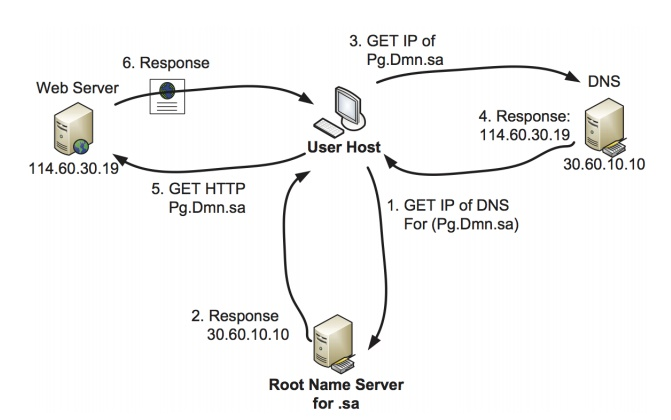
\includegraphics[scale=.7]{img/normal_FF.jpg}
single flux\\
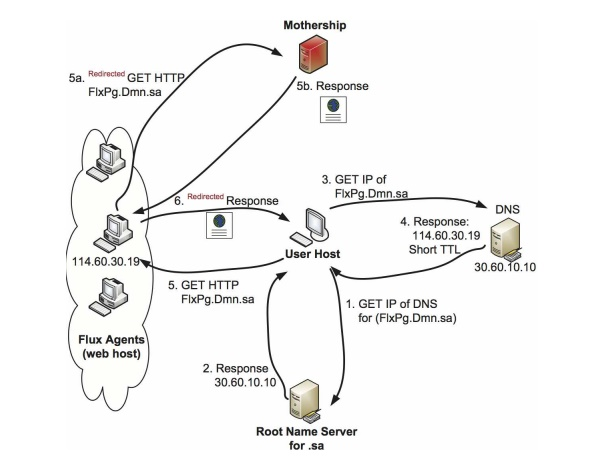
\includegraphics[scale=.7]{img/single_FF.jpg}
double flux\\
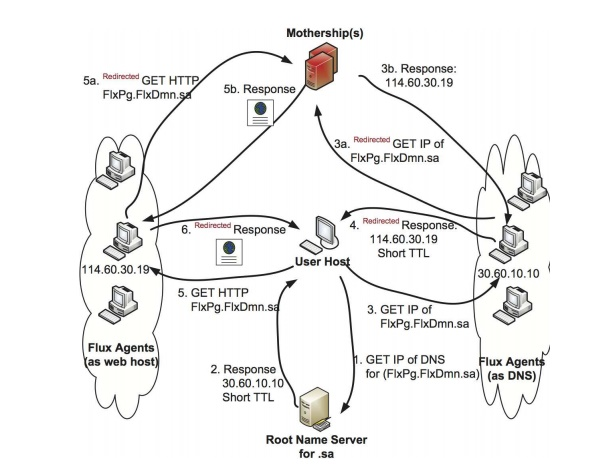
\includegraphics[scale=.7]{img/double_FF.jpg}


ADD IMAGE HERE:
\cite{ff_visual}
\cite{ff2_visual}



\subsubsection{DNS tunneling}
DNS tunneling is a technique used to bypass restriction on a protocol or hide certain activity by embedding it in the DNS protocol. For example using the TXT  as q\_type or the subdomain itself to actually carry encoded data (i.e bWFsd2FyZQ.maliciousdomain.com, where bWFsd2FyZQ is encoded text). Usually, the payload will be fragmented to avoid unusual long domains or packets. This has been done to avoid restrictions but botnets also use it to hide malicious traffic or payloads. They can also use DNS tunneling to remain undetected \cite{Botnet1} while exfiltrating data. The only positive aspect about this abuse is that there are almost no legitimate reasons for this application as we saw with fast-flux, this makes obvious malicious behavior stands behind if this type of traffic is discovered.\cite{tunneling}
\\
Paloalto's research unit provided a nice overview of the DNS tunneling practices\cite{tunneling2}. They explain how the protocol can be used either to exfiltrate or infiltrate data with infected machines. They show how different parts of the protocol can be exploited. They divided the botnet traffic using dns tunneling into 3 types: heartbeat, exfiltration and infiltration. A heartbeat will be a simple query for an A record met with a NXDOMAIN response. An exfiltration can only use the query to send data therefore, it is usually fragmented through multiple A queries with the data embedded in the query as mentioned above. A big problem remains that because DNS uses UDP it can't rely on the same assurances provided by TCP. And finally infiltration, this usecase has a lot limitations then the exfiltration because it can hide the encoded data in the values of the records such as the TXT record. It has the same problem as the exfiltration which it can't rely on the protocol to ensure the data is correctly arrived.
An interesting question they ask is how does the bot know when to ask for a TXT record instead of a A record. An they use a lot of different options but the most common one is the following: the malicious DNS server will respond with a NOERROR response when it is ready to provide the next payload and that is how the bot will change its next query for a TXT record.


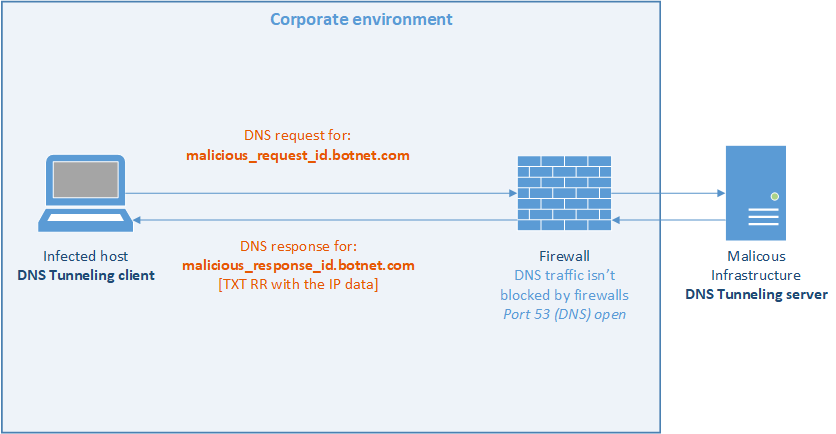
\includegraphics[scale=.8]{img/pers_tunn.png}


\subsubsection{Domain shadowing}
The last abuse of DNS which has been recently detected, used by botnets as a communication channel is DNS shadowing. DNS shadowing is an abuse obtain by stealing account credentials from legitimate domains for the purpose of creating subdomains aimed at malicious servers. This provides criminals with a great amount of subdomains that inherit their parent's domain reputation. This allows to bypass a lot of features based on reputation and 2LD.
Malicious actors cycle through the creation of subdomains which they delete shortly after, similar to the fast-flux rotation behavior.
\\
The reason this type of activity spawned is due to IDS using detection based on reputation scores for the domain names flagging domain fluxing and fast-fluxing making it complicated for botmasters to use those evasion systems as much. Malicious actors realized they could bypassed most detection systems by using the reputation of legitimate domains and that is when they started campaigns to harvest this specific type of credentials.

\cite{review2}\cite{detection8}

\cite{shadowing2}
\cite{shadowing3}
\cite{shadowing4}
\cite{shadowing5}

\section{Machine learning approach}
We use machine learning in our thesis to create models around certain behaviors botnets show to help us distinguish them from the legitimate traffic. The next sections will detail what machine learning is, how it works and its implementation in the thesis.

\subsection{Machine learning}
Machine learning (ML) is a mathematical study of algorithms and statistics that allow to learn and improve a certain task without being directly programmed. The goal is to improve the performance of specific tasks by building models of the problems. \cite{ml-def}

\subsection{Machine learning for botnet detection}
The goal of botnet detection is to distinguish between 2 classes of traffic: normal and malicious. We are interested in one of the tasks that machine learning algorithms excel at which is classification. After training the models, called classifiers, they are able to assign classes to any new data.
\\
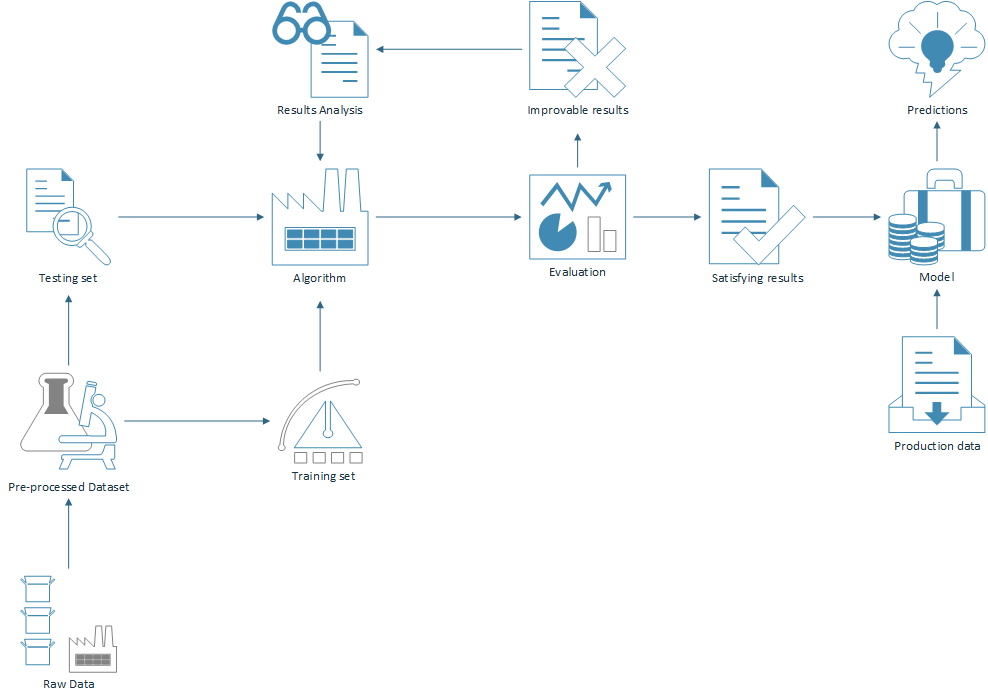
\includegraphics[scale=.4]{img/pers_ml_workflow.png}

\subsection{Machine Learning workflow}
Machine learning has a specific pipeline that needs to be followed to obtain the best results\cite{ml-workflow}: Gathering the data, selecting the features, extracting the features, choosing the right classifier, training and testing the model, and finally, assessing the prediction capabilities of the model. Each step is explained below and its implementation will be detailed in the experiment chapter \label{experiment}.

\subsubsection{Data gathering} The machine learning algorithms need to be fed data that has information about the problem. We need data that will be able to shape and create the model. In our case, we searched for captures of DNS traffic available publicly to study botnets, preferably labeled data as malicious or botnet. This labeling is essential for the learning stage. Another step which is important when creating the dataset is to balance it out correctly between the 2 labels. If there is an imbalance, the label with the greater presence in the dataset will influence the model excessively and poorly train it. The dataset research will be detailed in \label{datasetchapter}.

\subsubsection{Data pre-processing} 
Data pre-processing involves a number of processes, it aims at improving the quality of the data and depends on the type of data in the dataset. Its 2 main processes are feature selection and feature extraction. The feature selection consists on deciding what elements of the data are relevant to create the model and feature extraction consists in cleaning the data and formatting it correctly to be ingested by the machine learning algorithms optimally.\\\\

\paragraph{Feature extraction} It is important to realize that algorithms are programs that only understand numerical data. The raw traffic captures can't directly be ingested by the algorithms, these can only digest 3 types of formats: numerical (TTL value for a RR), categorical(DNS record types such as A, AAAA, TXT, CNAME, ...) and ordinal (short, medium, long). These formats can always be converted into numerical values which is the only thing algorithms can use. It is important to realize that only features from the data convertible into one of these formats will be able to be used. Format isn't the only thing that is important, with large datasets, we need to get rid of all the noise that they might contain as well as find missing data or inconsistency in parts of the traffic.
This section will be detailed in \label{featureextractionlabel}

\subparagraph{Feature extraction techniques} To clean and extract the features from the raw data, there are common techniques used. \\
The first is \textbf{conversion of data}, this consists in transforming the categorical and ordinal features into numerical ones (i.e [high, medium,low] would become [2,1,0]). This can even be improved by using hot encoding which creates a feature for each value of the category. Hot encoding is nevertheless mostly used for large categorical features.
\\
The second consists in dealing with \textbf{missing data} by either removing it or using an average for that feature not to have it influence the other data for that feature.\\
Thirdly, \textbf{anomalies} due to human errors for example need to be discovered and corrected manually.\\
Another aspect to consider are the scales of the features. Certain algorithms will give more weight to features that have a higher scale which would create a bias in the data. To deal with scale issues between the features there are two used techniques: \textbf{Normalization} and \textbf{Standardization}. \\
We normalize the features\cite{ml-norm} by dividing them by the maximum for that feature. The goal of the normalization is to avoid features unbalanced analysis by the algorithms. Features such as TTL with a range of values in [300-86400] compared to features such as the number of resolved IPs with values in this range [0-15], the difference in scale could have more weight in the algorithm due to the scale difference of the features. The normalization will project the features into ranges between 0 and 1. This makes the models less affected by scales and improve their learning.\\
Standardization aims to achieve similar results as normalization but through another method. It works by re-scaling the data so it has a mean of 0 and a standard deviation of 1. Standardization is shown to improve comparison between features with different units and scales as well as make the training process better for the classifiers.
\\
As explained in this article\cite{normstd} normalization and standardization seem to always improve quality of the results but the choice of scaling function can have important different results. Therefore, this is why will will test our results using the different scalers available for each classifier.

\paragraph{Feature selection} \label{featureselectionlabel}is an important step of the workflow. The choice of the data that will be ingested is crucial and directly connected to the results we will obtain. We can select features based on pattern or data type.\\
Pattern based selection means through the statistical analysis of the data and using unsupervised learning algorithms to extract tendencies from the results. This aims at finding patterns for each label and understand the underlying reason. \\
Data type based means that we focus on the specific features related to the traffic from the labeled data. Most of these features have already been analyzed by other researchers and will be based on the nature of the DNS traffic coming from malicious or normal labels.\\
\\
After you have chosen the features from your dataset, there are a couple of things to look for: The number of features used can be a major impact of your research in regards to redundancy of the features, complexity related to number of dimensions, overfitting the model. Our next step is to decide which features we want to keep for our experiment. \\
Here are some questions to help us in that selection.

\subparagraph{Are the features independent enough from each other to have a balanced weight between general features?} The problem that often arises in ML is that different features are providing the same type of information and not adding value. This can push the balance of the models in their direction and result in a biased model. There are multiple solutions used in ML for this issue:  analyzing feature correlation and removing strong ones, scatter mix plots to understand links between features and finally importance analysis through the use of the Random forests algorithm.
\\
\subparagraph{Are there issues with large sets of features?}
This is where we can see the curse of the dimensionality manifest itself. Where problems such as exponential computing and overfitting come in to play. Some machine learning algorithms handle large sets of features very well but others have an exponential complexity when it comes to the number of features and it can end up slowing your research process. The problem of overfitting is important to take into account when doing ML and keep in mind that our dataset might not represent the global view of the problem we are solving. This means that if we create a model that doesn't generalize enough it won't work on other data as well even if you obtain really good results.\\
To solve dimensionality there are a couple of solutions, some are part of reducing the amount of features by removing the less independent ones or important ones. There are other solutions such as Principal Component Analysis (PCA) and Linear Disciminant Analysis(LDA)\cite{ml-reduction}. \\
PCA is a procedure that transforms a group of features that could be correlated into linearly uncorrelated features. The features provided are named principal components and provide valuable features for model creation but they are also hard to interpret. Its use introduces a part of shadow in the results which is a trade-off to take into account when using it. \\
LDA models distributions of the features given into classes then uses Bayes to estimate their probability, it is mostly used in ML for dimensionality reduction.\\
Both are similar in the way that they look for the best way to explain the data they are given.
\\
\subsubsection{How to chose the right algorithms?}
To answer this question we first need to learn which are the differences between the available algorithms and what they look to achieve: 

\paragraph{What are the different machine learning categories of algorithms?}
There are three mains categories of algorithms in machine learning based on their learning method: supervised learning, unsupervised learning and semi-supervised learning.
These categories are based on the training data given to the algorithms. \textbf{Supervised algorithms} are provided labeled data, they analyze the features and learn what characteristics are proper to each label. This is how the classifiers build models to predict the labels for new data.
\textbf{Unsupervised algorithms} use unlabeled data as input. This type of algorithm will group data based on similar values for different features.
Semi-supervised algorithms is the combination of both, where the training data is partially labeled. This is very useful for datasets where there is only partial labelisation available.
\\
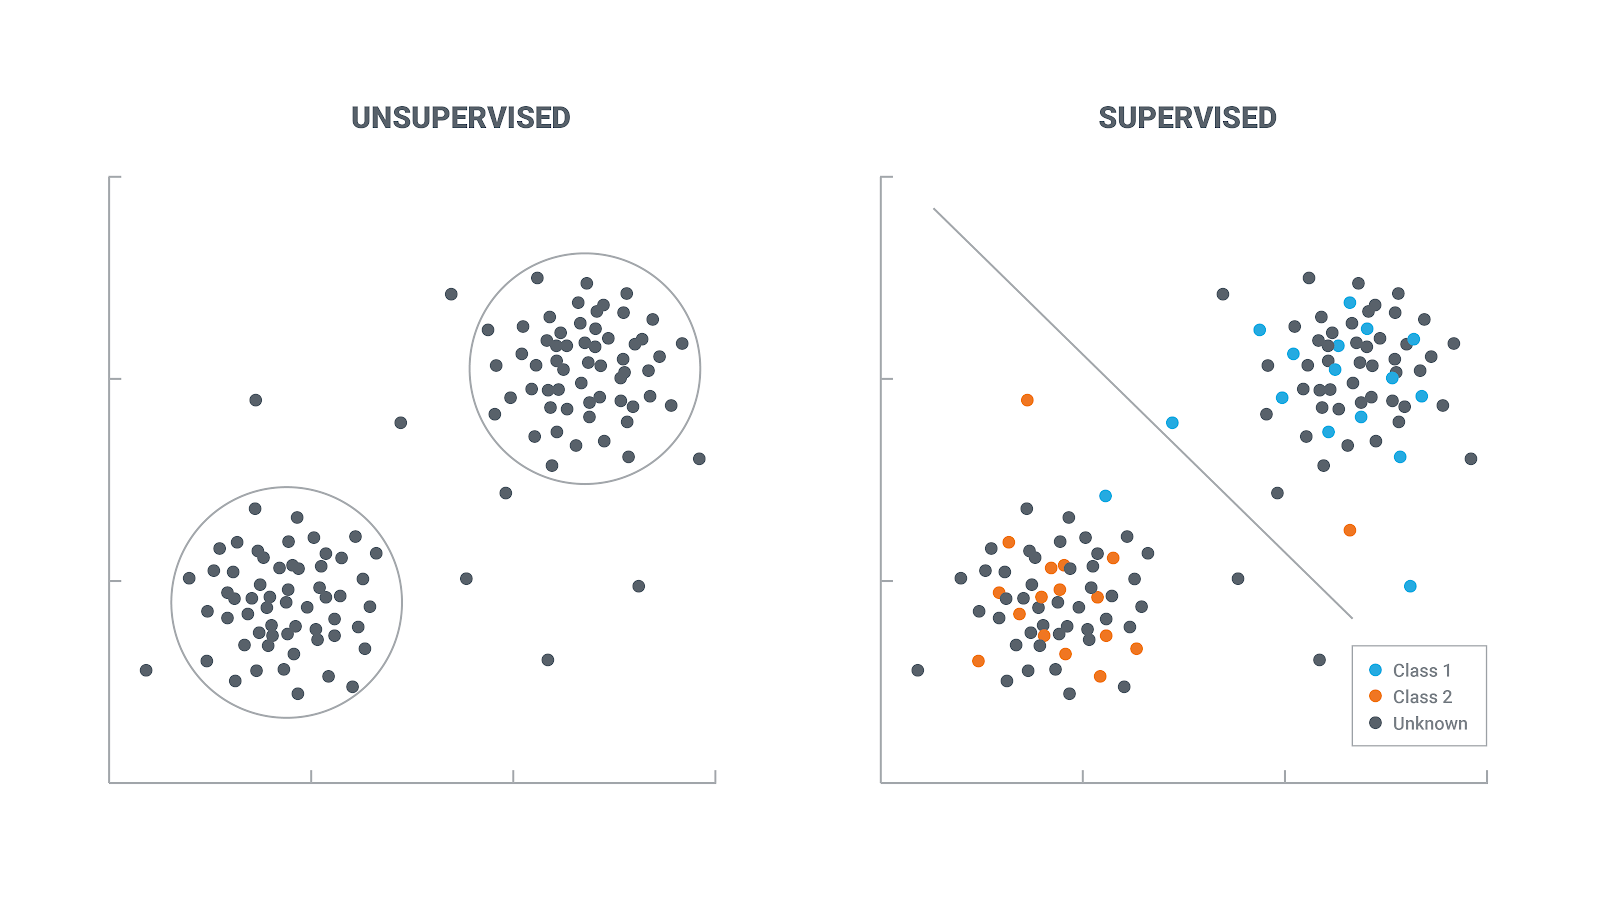
\includegraphics[scale=.3]{img/supVsUnsup.png}
\cite{supvsunsup}
Now we need to decide what algorithm makes more sense to model the data in accordance to the problem that is being solved. We are trying to solve a detection problem. This  falls into a classification problem where supervised algorithms prevail\cite{supvsunsup2}. To find the best algorithm to model the problem we will test out different algorithms and compare them under the same conditions.\\
\\
TODO: decide if we do this?
%Supervised algorithms have been chosen for the modeling part of the problem but unsupervised of algorithms will be used as well for the research of new features in the \textbf{features selection} step.

\subsubsection{Training the models}
After the steps above, we have a balanced and clean dataset, we have the features that will be used to model the classes and we have a list of algorithms.
\begin{enumerate}
\item Now comes the part were we are going to feed this data into our algorithms and start creating a model. The way models are verified is by dividing the dataset into 2 sets, one for training and one for testing. The way datasets are divided into the 2 sets are up to us, the standard is 80\% for the training set and 20\% for the testing set. The choice is ours, as long as the testing set is large enough to provide accurate statistical results and is diverse enough to be a good representation of the rest of the dataset.\\
\item Each algorithm possesses parameters which are called hyper-parameters, that allow us to fine-tune the algorithms to the problem and the data. However, it would take a very experienced data scientist to be able to manually set those parameters correctly. For problems with small dimensions, the model can be visualized and it becomes easier. In our case, we have too many features to visualize the resulting model in a way that will help us understand what needs to change. For this reason, there are 2 main techniques that are used to help with this issue which are the \textbf{Grid Search} and \textbf{Random search}\cite{ml-search}. \\ 
The grid search selects a set of values for each parameter and then runs the training of the model each time with a different combination until they are all covered. The output is the combination of parameters with the best accuracy score. This disadvantage of the technique it is affected by the curse of dimensionality. \\
The random search works similarly but instead of trying all the value in the range of the parameter, it randomly picks a subset of combinations. For lower dimensional problems, random search has been proven to perform better.
\item To validate the performance of the trained models in the least biased manner the machine learning community uses a technique called the k-fold cross validation\cite{10-fold}. For each one of the algorithms, the training set is divided into k random folds(equal subsets). One of the folds is then chosen as the testing fold and the rest as training for the algorithms. The algorithm is trained and tested. We repeat this process k times until all the folds have been used as the testing fold. This provides the best classifier able to generalize the data in the training dataset. It is important to point that for classification problems, we use a variation which is the stratified k-fold cross validation, this technique ensures that through the folds the balance of classes keeps the same proportions. The common value for k is 5 or 10. The results obtained are a realistic and unbiased representation of the model's performance.
\end{enumerate} 
\begin{figure}[h]
\centering
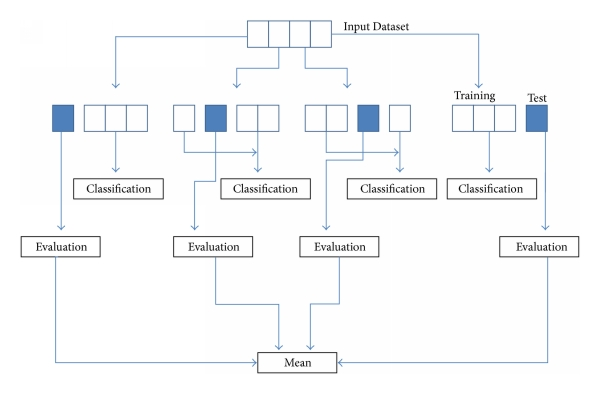
\includegraphics[scale=.3]{img/K-fold-cross-validation.png}
\caption{An example graph}
\label{fig:x cubed graph}
\end{figure}

\subsubsection{Testing the model}
We now have obtained a classifier, we need to see how to performs with our testing set. The process is pretty simple, we take the classifier and give it our testing set as input, it is important to know that the set provided to the classifier are the features only, the testing set given to the classifier isn't labeled. The result is the labeling of the testing set. From this point, we enter the analysis of the results where we compare the resulting labels from the real class they belong to.

\subsubsection{Analysis of the model's results}
In this section, we will use the metrics obtained from the results of the model's predictions to provide us information on the experiment and to enable the feedback loop. For classification problems, the most common technique is the confusion matrix which can derive a large number of useful metrics including accuracy, precision, recall, F1-Score. There are also other advanced metrics \cite{ml-metrics} that can be introduced such as: Logarithmic Loss, Area Under ROC Curve and more. All will be described in the result chapter.
These metrics will help us understand what can be improved and if the direction we are taking is improving or not the model. From there we will adapt the features and the parameters of experiment to improve the results. The goal is to reach the best results possible.

\subsubsection{Result interpretation}
The last part of the experiment is the interpretation of the results. We want to understand how our classifier works. To do so, we have at our disposal tools such LIME, SHAP, RFs and more that help us understand which features are important and what are the model's behaviors\cite{ml-inter}.
Those tools will be defined more in depth in the result's chapter, under the interpretation section.

\subsection{How will machine learning be implemented for this Thesis?}
TODO: Review the need of this section.\\
A big part of the work will be the feature selection. Going through the papers that have already done research on the subject, doing statistical analysis and using unsupervised learning to possibly extract more features and pick the ones we consider most effective. The algorithms used for detection as well as their parameters, are an important aspect of the experiment. A big part of the challenge in machine learning is to find the features with enough strength to create the model and the right settings for the classifiers so the fit the data correctly, it is very easy to fall in the over-fitting or under-fitting problem.

\subsection{Algorithm selection}
Based on the explanations above on how to chose the right algorithms, here we present the algorithms we will use. The reason for picking them is their mainstream use for this type of problem.

\subsubsection{Gaussian Naive Bayes}
This comes from the know probability and statistics Bayes' theorem. "It describes the probability of an event , based on prior knowledge of conditions that might be related to the event"\cite{bayes}. In ML learning the model saves the probabilities of each feature to belong to which category and when it is asked to predict new data, it does so by computing the event's probability to belong to each one of the categories. It bases its predictions on previous experience.

\subsubsection{K-Nearest Neighbors}
k-Nearest Neighbors (kNN) is a very simple supervised ML algorithm. kNN classifies new objects based on their nearest neighbors. The parameter k represents the amount of nearest neighbors it looks for before it assigns the majority. The model created by kNN is actually the entire training dataset since it will use all the neighbors to determine the classification of a new item. kNN algorithm works well with a low amount of features, with datasets with large dimensions computing the distances for the k-nearest neighbors becomes computationally expensive.

\subsubsection{Decision Trees}
Decision Trees(DTs) are supervised algorithms that based on observations of labeled data creates a model of decision that is represented by a tree where all the nodes of the tree are a condition for the features and where all the leaves are the label they are classified as. The classification process starts at the root and ends in one of the leaves.\\
DTs are very simple to visualize and perform really well even in higher dimensions. The most common problem of DTs is the overfitting of the data. Because outliers and unbalanced datasets will create branches that don't generalize the data correctly.

\subsubsection{Support Vector Machine}
Support Vector Machine (SVM) is a supervised algorithm that excels in classification problems. The algorithm looks locally between the classes what hyper-plane separates them. 
Its hyper parameters are very interesting too, they allows to adapt to the dimension of the features to allow for transformations of the hyper-planes relative to the dimension. They also allow to tune how much we accept outliers. The tuning has to be done with care because we could end in an overfitting situation that doesn't generalizes enough and therefore could perform poorly with new data.

\subsubsection{XGBoost and Adaboost}
Both algorithms, eXtreme Gradient Boosting (XGBoost) and Adaptive Boosting (AdaBoost), are based on a similar concept which is boosting. Boosting is a technique that modifies weak learners into strong learners. It is done by training multiple of these weak learners sequentially and each improving based on the previous one.\cite{boosting} Both use this technique with different approaches to it.

\paragraph{AdaBoost}
The boosting used with Adaptive Boosting(AdaBoost) is simpler than XGBoost, it uses decision trees with a single decision node, they are called decision stumps. Each mistake made by stumps during classification are forwarded to the next stump by carrying more weight. This will allow the errors to be corrected of the numbers of stumps and obtain a cleaned up result in the end. This concept is mostly applied with DTs but it could be applied to any supervised algorithms. As are trees, AdaBoost are victims of outliers but they do a good job not to overfit the models as its peer. 

\paragraph{XGBoost}
The type of boosting used with XGBoost is Gradient Boosting on steroids. The algorithm improved is the RFs which is already a really strong supervised classifier. Like the AdaBoost, it sequentially improves the current tree using its predecessor but instead of adding more weight to the misclassified observations, it tries to train the next predictor to those observations. But this isn't all, XGBoost was created for fast and high performance to solve the slow characteristic of gradient boosting. That is where the eXtreme part comes in and where they introduced solutions to its shortcomings: parallelization of the tree construction,  distributed computing, out-of-core computing and cache optimization.\cite{xgboost} Due to this, it is one of the most popular algorithms because it provides the best performance on a range of difficult machine learning tasks. Its only drawback is its overfitting but that can be solved fine-tuning its hyper-parameters and it's explainability which can be complicated.

\subsubsection{Random forest}
The Random Forest (RF) algorithm is an improvement of the DTs. The concept is to randomly create low correlated models (forest) and give them the same input. It then picks the majority result as the prediction for the input. This technique provides a good way to protect from the overfitting that DTs are known for and to protect against individual errors of the trees. RF takes advantage of Bagging (Bootstrap aggregation) and Feature randomness to achieve this uncorrelated forest.
Bagging consists in giving all the trees the same amount of data but with replaced data (duplicates). Secondly feature randomness as its name implies, at each node the trees only take decision based on a subset of features.\cite{rf}

\subsubsection{Artificial Neural Networks}
Artificial Neural Networks (ANN) is an algorithm created similar to how the brain works and its learning capabilities by modeling neurons and their synapses. It works as a black box system with inputs on one side and and outputs on the other which are dependent on the inputs. The black box is a network of neurons grouped in layers, neurons of each layer connect with the ones of the next layer with weighted connections that will determine when the neurons fire. The modeling is around finding the values of the neurons and the connections inside the blackbox (hidden layers). The way ANNs hidden layers are computed are through gradient descent, a way of automatically updating the weights step by step into a direction that will make them less wrong, based on the output desired.\cite{ann}

\section{Classification of botnet research and detection}
In this section, we are going to present the current state of the botnet detection taxonomy and show the weaknesses and strengths of each method. This will be followed by a discussion in the next chapter of the current state of the art when it comes to passive traffic analysis for botnet detection and what we are going to bring to it. 

\subsection{Taxonomy of Botnets}
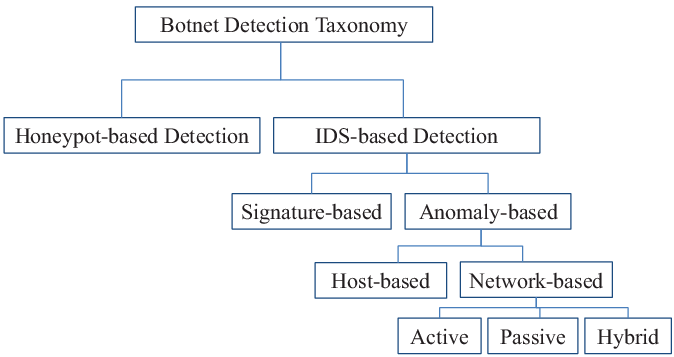
\includegraphics[scale=.6]{img/Botnet-detection-taxonomy.png}
\label(taxonomy)

%%%% SYSTEMS
\subsubsection{Detection systems} In a recent survey, Alieyan et al. \cite{survey1} presented the taxonomy of botnet detection techniques. We will follow down the path of the detection taxonomy until reaching our center of interest. As we can see on the figure \ref{taxonomy}, there are 2 type of systems used for detection: \textbf{Honeypots} and \textbf{Intrusion Detection System} (IDS). Honeypots aim at creating an environment specially forged to attract malicious traffic and extract information from the behavior of the malicious actor on the host. IDS aim at analyzing the network and security logs, and alert the security analysts of any malicious or suspicious traffic. The IDS is divided into 2 techniques. An older one \textbf{based on signatures} and newer one \textbf{based on abnormal behavior}.

%%%% IDS
\subsubsection{A legacy problem} A big trend among companies for a long time and even today was solely use of a signature-based detection in their IDS \cite{detection8}. However, these signatures have shown to be ineffective against bots that are constantly getting updated with new code and new evasion techniques. Furthermore, they are ineffective against any new type of emerging botnet. Signature-based detection is great for known botnets\cite{snort} and should always be implemented in IDS solutions but is insufficient and should always be coupled with other techniques. The recent introduction of other techniques such as abnormal behavior has been mostly motivated by the goal to solve this issue.

%%%% ABNORMAL BEHAVIOR-BASED
\subsubsection{Where are botnets detected?} In the anomaly detection technique, researchers have found relevant data in different locations: directly on the host affected and throughout the network the host belongs to. Location wise, here are 3 types of behaviors observed from bots\cite{bot-threat1} :
\begin{itemize}
\item \textbf{Network based behavior}: this is the observable network traffic between botmaster and bots. The goal is to uncover the communication channels and any traffic related to attacks. 
\item \textbf{Host based behavior}: observable activity on the host infected by the botnet. This activity is mostly what Antivirus (AV) software cover.
\item \textbf{Global correlated behavior}: This focuses on the global characteristics of botnet behavior, they focus on fundamentals structures of the botnets that could emerge and be used for detection.
\end{itemize}
Since AVs already provide coverage of the host-based behavior, we have decided to focus on the locations where IDS still have a lot of room for improvement, we focused mainly on the network aspect because obtaining data to analyze global network correlation isn't easily obtained.

%%%% PASSIVE APPROACH
\subsubsection{What are the types of approaches for network behavior detection?}
They are classified into 2 categories: \textbf{passive detection} and \textbf{active detection}\cite{detection9}. \\
Passive detection consists in gathering data through monitoring logs. Activity on the network is tracked without interfering with it, also making it harder for botmasters to notice it. This method is limited in the amount of data it can gather. Some examples of this approach: deep packet inspection through IDS, flow records analysis for traffic flow pattern identification, DNS monitoring, spam records analysis for botnet correlation, application log files analysis.\\
Active detection differs from the passive approach by interacting directly with the information it observes. Because of the changes it may introduce, this approaches can be detected by the botmaster that might change the behavior of the botnet or add elements of evasion. There are 2 main examples: Sinkholing, this consists in redirecting the traffic of the botnet to a controlled machine to cut off the CnC, and Infiltration, which tries to wiretap or take control over the botnet from the inside by reverse engineering the malicious code and traffic. Other examples of active detection: FFSN tracking, IRC traffic analysis, peer-to-peer networks enumeration.
\\\\
Everything presented above applies to all botnet using different protocols. The interest to study this part of the taxonomy, particularly the DNS passive traffic approach comes from the progress it has shown and the large amount of possibilities that still can be studied.\\
Let us now analyze the particularities of the DNS passive traffic analysis.

\subsection{Passive DNS detection Techniques}
\paragraph{What are the different passive detection methods?}
With the DNS logs captured, researchers have proposed different approaches to utilize them, most of the methods involve a statistical analysis or the use of machine learning algorithms to create classifiers. Others have opted for detection through visual representations to detect anomalies.\\
The reason we have decided to focus on the machine learning approach as mentioned in the introduction is two-fold: a will to develop our machine learning skills and methodology but also because botnet detection state of the art has shown it to be the most effective method, achieving better scores then the other techniques in the taxonomy.\\
As explained in the "abuse" section of the DNS chapter, a new type of detection techniques have been studied that aim at finding bots using the DNS protocol to evade the more usual detection techniques which is what we aim to further study and hopefully improve the current solutions.

\section{Related work}
Our end goal is to find the best features and techniques possible to improve the current solutions that aim at detecting all the evasion techniques, that we have named \textbf{Combined Solution}. To do so, we have structured our research as follows:\\
First, we will present the combined experiments. These experiments do not focus on a single type of detection mechanism but aggregate the different detection techniques used by botnets. We will discuss the features they have extracted, what models they have created and how they have implemented their approach.\\
Secondly, to achieve our goal towards improving these solutions, we will discuss the weaknesses of their approach and how we plan to improve it.\\
Thirdly, we will present the current state of research, the studies that we have used to improve the solutions. To structure this part we have divided the related papers by evasion technique.
The objective is learn the different approaches from different papers, find better features and better models, see which we think could improve the current solutions and then test them out in our experiment.

\subsection{Presentation of the Exposure and the Local botnet experiments}
The first step in the research was to find the models that would be the current baseline for all-in solutions: because it is considered as the best all-in solution paper we could find, we are going to compare and extend the work of the EXPOSURE team.

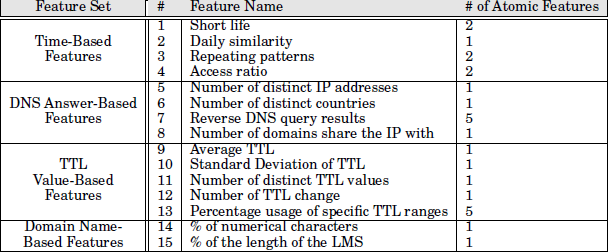
\includegraphics[scale=.8]{img/exposure_features.png}
\includegraphics[scale=.8]{img/exposure_architecture.png}

\paragraph{Time-based}
When we analyse many requests to a particular domain over time, patterns indicative of malicious behaviour may emerge.\\
These were supposed to be the features with the most weight, unfortunately due to lack of the same caliber of capture available to the authors of Exposure, we could not test out the 4 features related to time. Either because the datasets are compositions of smaller datasets, or because the timestamps are too short.
\paragraph{DNS answer based}
Here are some domain-flux features: A domain name can map to multiple IP addresses. In such cases,the DNS server cycles through the different IP addresses in a round robin fashion and returns a different IP mapping each time. \\
Malicious domains typically resolve to compromised computers that reside in different locations. The attackers typically use domains that map to multiple IP addresses, and IPs might be shared across different domains.
\begin{itemize}[noitemsep]
\item the number of different IP addresses that are resolved for a given domain during the experiment window
\item the number of different countries that these IP addresses are located in
\item the reverse DNS query results of the returned IP addresses
\item the number of distinct domains that share the IP addresses that resolve to the given domain (false positive can be reduced with google reverse DNS which will have hosting providers in top answers)
\end{itemize}
\paragraph{TTL value based}
Low TTL and Round-Robin DNS: \\
\begin{itemize}[noitemsep]
\item high availability (Content Delivery Networks (CDNs))
\item botnets using this, makes them resistant to DNS Blacklists(DNSBL) and take downs. Often using Fast-Flux Service Networks (FFSN).
\end{itemize}
Because FFSN are usually detectable because of low TTL and growing list of distinct IP addresses for a domain, it explains the purpose of the TTL features.
\paragraph{Domain name based}
Finally 2 simple features to expect detection of DGA: there is a big difference between legit domain names and domains generated by DGAs(Domain Generation Algorithms(DGAs).\\
This can be noticed with 2 simple features:\\
\begin{itemize}[noitemsep]
\item ratio numerical chars to length of domain name
\item length of the longest meaningful substring to length of domain name
\end{itemize}



Heuer et al.\cite{localbotnet} did a case study on local infections related to botnets. They propose a very large set of 24 features meant to detect botnets in networks . These features aim at the different evasion techniques that are used by botnets and the purpose is to be able to detect any form of Botnet in the network analysed.\\
features:
\begin{tabular}{c|l}
\hline
 & LMS\\
Domain-name based & numerical / character\\
& Ngram\\
\hline
 & DBForwardBackwardSimilarity\\
DNS-based & DBDialup\\
& Nb distinct IP addresses\\
& Nb distinct Countries\\
& Nb distinct Domain Share IP\\
& NXDomain\\
& MXRecordPresent\\
& SOA (min, exp, refresh, retry)\\
& TXTRecordLength\\
\hline
 & Nb distinct AS\\
AS-based & Reputation AS\\
& Size of AS\\
\hline
 & Daily similarity\\
Time-based & Repeating patterns\\
& ShortLife\\
\hline
 & Average TTL\\
TTL-based & Nb distinct TTL values\\
& Nb TTL changes\\
& \% usage of TTL ranges\\
& Std deviation TTL\\
\end{tabular}

\subsection{Weaknesses and possible improvements}
TODO: rework this section.
These features are very specific to each mechanism and only work on the botnets that use them. That is why in the second part, we presented solutions with combined approaches. We want to experiment if a combined solution could provide better results and have other advantages such being more effective against new families of botnets. 
This type of project already exist such as the project Exposure detailed above. The detection rates obtained by Exposure are really good but they are hard to implement in a real environment because the time-based features are hard to obtain. Furthermore, in their study they showed that these features were the strongest features of the set. This means that without the access to these features their experiment doesn't show the same level of success. What we aim to do in our experiment is to provide smaller environments with similar detection capabilities as Exposure but with the features available in smaller environments. 

TODO: weaknesses and improvements found in the other combined approaches.
\subsection{Focused experiments}
Here are research papers that have proposed different techniques to detect botnets using these different evasion techniques presented in the abuse section of the DNS chapter. These are the papers where we found features and ideas to improve the above experiments. For clarity, we have divided them by evasion mechanisms.
\subsubsection{Domain-flux}
Domain-fluxing detection is mostly about analyzing domain names, here are the papers that attempt to do that with different metrics and features.\\
\\
Truong et al. \cite{dns-traffic} came up with an experiment allowing them to detect domains generated by humans or algorithms. This is the base-ground study of DGA detection.\\
\\
Yadav et al. \cite{dga2} propose an unsupervised approach based on anomaly detection with a set of metrics analysing ngrams of the SLD. They use the Kullback-Liebler divergence measure with uni-grams and bi-grams, the Jaccard index between bi-grams and the last feature and the Edit distance. These 3 features are used widely in the DGA detection research because of their efficiency.\\
\\
Schiavoni et al. \cite{phoenix} go a step further then Truong et al. with their Phoenix project by improving the initial experiment with additional features to cluster groups of DGAs under botnet families. The project works in 2 phases: DGA discovery and DGA detection. In the discovery phase, they apply the following filters that focus on linguistics: percentage of meaningful words in the domain name and the popularity of the n-grams of the domain. They construct a base generated with the top 100.000 domains from \textit{alexa.com}. Then define the Mahalanobis distance and the thresholds, using known malicious domains,  to determine when domains can be considered DGAs. Their approach is able to associate new DGAs to botnet families and follow their evolution.\\
\\
Ahluwalia et al. \cite{dga} analyse the basic features that are common to most domain generated by DGA and provide advanced linguistic features to improve the results. The motivation for their work was due to recent botnets using shorter DGA lengths to blend with the other domains. They then propose 3 primitive features that capture linguistic and structural characteristics and 2 more advanced features that cover the shortcomings of the primitive ones. These features are simple but obtain really good results.\\
\\
Antonakakis et al. \cite{dnsreputation}, in this paper they propose a different system called 'Notos' based on dynamic reputation odd domain names. They studied the different aspects around the historical DNS data of domains that could be relevant to group domains based on their legitimacy. They use 3 categories of features: network, zone and evidence. They opted for a unsupervised approach using the clustering algorithm X-means. The purpose of this paper is to utilize some of the historical DNS features to be used in our all-in solution. Specifically, using some of the classes of domains defined by the authors as categorical features ( popular domains, common domains, Akamai domains,  CDN domains and dynamic DNS domains ).
\\
Thomas et al. \cite{dga4} realized that during the domain generation process, most of the domains will not be up. This should result in a lot of NXDomain responses. Furthermore, the caching of NXDomains is limited which means that they cannot hide this traffic. Their contribution consists of a clustering technique based on domain names and request patterns; and similarity metrics for malicious domains detection.

In another paper from Yadav et al. \cite{dnsfailure}, they explore the detection possibilities in the DNS failed queries due to the fast fluxing behavior. Botnets are querying a large number of domains which are only up for specific amount of times, this results in NXDOMAIN responses from the DNS queries emitted, their research has tried to use this information to improve current detection systems.

A similar idea was proposed by Antonakakis et al. \cite{pleiades} creating Pleiades, their second big botnet project after the Notos experiment. First, following the same machine learning idea of Notos but applied to the DGA algorithms, meaning they applied the X-means clustering algorithm to DGA algorithms. Secondly, they used a boosted decision tree classification algorithm (Alternating Decision Tree) to test associations of an NXDomain's response to  DGAs. Finally, they created Hiddem Markov models for each of the DGAs domains to be able to classify the responses to a DGA directly. We'll use their work to improve the DGA features already gathered with the other papers.

%P1 Mean, median and standard deviation of 1-gram
%P2 Mean, median and standard deviation of 2-gram
%P3 Mean, median and standard deviation of 3-gram
%P4 Mean, median and standard deviation of 4-gram
%P5 Mean and standard deviation of entropy(d)
%P6 Mean and standard deviation of entropy(2LD)
%P7 Mean and standard deviation of entropy(3LD)
%P8 Mean, median, standard deviation and variance of domain name length
%P9 Mean, median, standard deviation and variance of # of domain levels
%P10 Number of distinct characters
%P11 Number of distinct TLD
%P12 Ratio of .com TLD
%P13 Ratio of other TLD
%P14 Mean, median and standard deviation of the occurrence frequency distribution for the different TLDs
%Table 8: Pleiades features

\subsubsection{Fast-flux}
The behavior of IP fluxing has been well analyzed by the community and most papers propose similar features to detect fast-flux. They often differ with different settings for their experiments. On the other hand, the big challenge for our thesis was to find the features that allowed us to find differences betweent malicious fast-flux networks(FFSN) and content delivery networks(CDNs). Both use fast-flux for different reasons making it hard to differentiate.\\
\\
The common features presented by  Salusky et al.\cite{honeynet}, Nazario et al.\cite{ff1}, Perdisci et al.\cite{ff2}, Holz et al.\cite{ff3} and Stalmans et al.\cite{ff_botconf} bring forward the features to detect fast-fluxing in general such as a large amount of unique A RRs for a domains, numerous unique NS for a domain and different Autonomous System (ASN) for the IPs linked to the same domain. \\
The next papers present additional features to distinguish detection specifically of the FFSN from the CDNs. \\
\\
Nazario et al. \cite{ff1} showed visually how the FF traffic features present themselves.
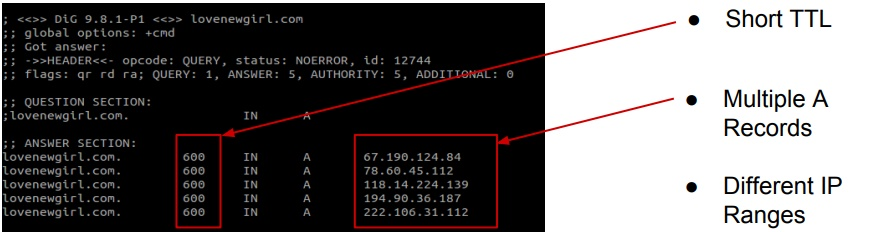
\includegraphics[scale=.7]{img/ff_features.jpg}\\
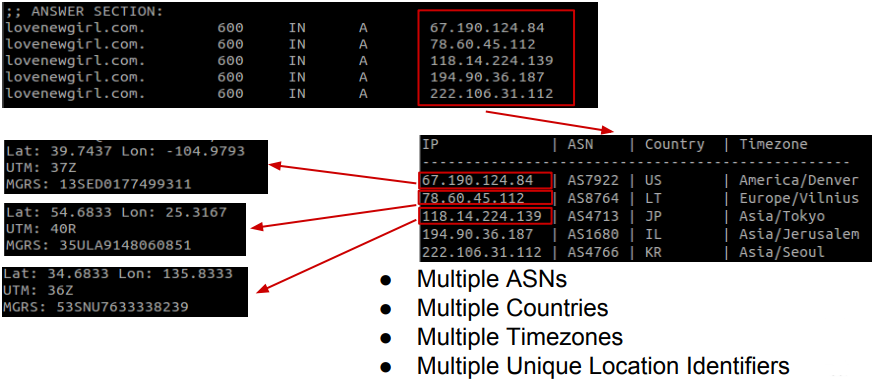
\includegraphics[scale=.6]{img/ff_features_2.png}
\\
Perdisci et al. \cite{ff2} aimed at improving the Honeynet's features \cite{honeynet}. Their method consisted in collecting recursive DNS logs for a period of time, filter most of the non-fast-fluxing traffic. Secondly, they grouped the domains names using different features such as similar ISPs, same CDN. And finally, they classify, using a Decision Tree algorithm, the clusters of domain names as malicious or legitimate. They used a base of features provided by \cite{fluXOR} and added their own. We used some of the features they presented for our classifiers as well as the traffic volume reduction filters to improve some of the features already on-boarded. \\
\\
In the following paper, Holz et al. \cite{ff3} propose some novel features compared to the other papers. They presented the restrictions FFSNs face compared to CDNs: problems such as location and uptime that FFSN can't garantee. From all the features they captured they introduced functions to classify FFSN and CDNs:fluxiness and flux-score. They even considered the possibility of botnets mimicking CDNs but the metrics used already take into account the restrictions FFSN have that can't be avoided. The rest of the study approaches the detection of FFSN using the HTML content returned by the spam websites. We focused our interest in the 2 functions presented in the paper as new features for our classifiers.\\
\\
Celik et al. \cite{ff4} have regrouped the large majority of features encountered in the other papers accompanied with some novel additions. They have 5 categories of features: answer-based, domain name-based, spatial-based, network-based and timing-based. We added to our list of features the ones we hadn't seen yet such as the spatial approach looking at the entropy of time zones related to A or NS records. The second interesting set of features we attempted to use in our thesis were the timing-based featured analyzing delays related to different actions (network, processing and document fetching) but we realized that we didn't have the capacity of building the infrastructure necessary to analyze them.\\
\\
TODO: Perdisci et al. \cite{ff} 


\subsubsection{DNS tunneling}
Another evasion technique of botnets that exploits the DNS protocol is the concealing of data exchanges through DNS tunneling. We explore below some of the studies that have proposed features and methods to detect such behavior.

In \cite{tunn1}, Dietrichyz et al. analyze the use of TXT RR with segmented and encrypted data. Their study resulted in a set of features mostly analyzing the strings characteristics. Rdata features: we look for the Shannon entropy of the strings. Measures the randomness of the string. Since encrypted data as a high level of entropy this is one of the things we'll be looking for. We are looking for "high byte entropy". Because of inherent reasons this entropy for a small string can't reach the max, we are looking at the "statistical byte entropy" instead. They expect these behavioral communication features to be effective enough in order to extend a classifier based on the rdata features.\\
\\
In this article written by G. Farnham \cite{tunn}, he proposed a visual approach to detecting DNS tunneling, by plotting the set of features proposed, you can detect by "visual anomaly detection" the presence of DNS tunneling in your network.. 
x-axis: destination IP
y-axis: character count
radius: hostname length
colour: request type

\url{https://vimeo.com/38727629}

IDEA: use the DGA tricks to plot some of the tunneling done
but more specific to NXDOMaINS / NO ERRORS and TXT / base64

TODO: This last paper \cite{dns-tun}

\cite{tunn2}

TODO: check if this is the same paper used to detect DGA, the study looks very similar. % https://pdfs.semanticscholar.org/c7cc/7c16e8952facae1e4dfb0dd768a4504cd5cb.pdf

\cite{tunn3} 

\cite{tunn4}

TODO: follows the same idea but visually.

\subsubsection{Domain shadowing}
TODO: Liu et al. \cite{shadowing} are the first to propose an approach against this new trend. 


\subsection{Value summary}


\section{Our botnet detection contribution}
In the first part of the related works, we presented Bilge et al. \cite{exposure} where they propose a large-scale system that uses passive DNS monitoring of 15 features to detect malicious activity. The interesting parts of this paper were some of the unusual features proposed among the 4 categories of features presented and their pipeline for the project which we used for inspiration. What we look add to this paper is the low-scale part that is missing, some of the features are only available to ISPs and the idea is to scale it to any company with DNS monitoring capabilities.\\
\\
The second part presented very interesting studies and projects that allowed the detection of the different evasion mechanisms using the DNS protocol. They allowed us to extract valuable features and techniques for each mechanism. \\
\\ 
TODO: Explain our possible contribution: 
"lower FPR, stronger features, better applicability of features, different modules"